\section{Introduction}
\begin{frame}
\frametitle{Introduction: Evapotranspiration (ET)}
\begin{columns}
	\begin{column}{0.5\textwidth}
		\begin{itemize}
		\setlength\itemsep{1em}
		\item Loss of water through:\\
			\begin{enumerate}
				\setlength\itemsep{1em}
				\item Evaporation and 
				\item Transpiration
			\end{enumerate}
		\item Applications:\\
			\begin{itemize}
				\setlength\itemsep{1em}
				\item Irrigation scheduling
				\item Water resource planning, etc.
			\end{itemize}
		\end{itemize}
	\end{column}
	\begin{column}{0.5\textwidth}
		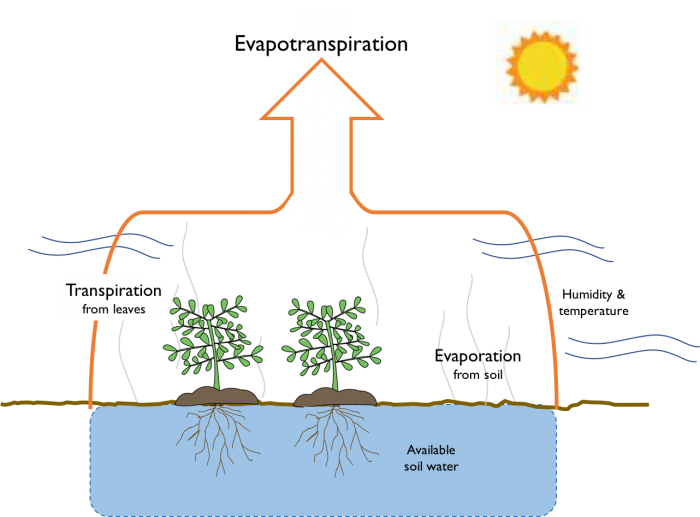
\includegraphics[width=\textwidth]{images/evapotranspiration.png}
	\end{column}
\end{columns}
\end{frame}

\begin{frame}
\frametitle{Introduction: CIMIS Weather Stations}
\begin{itemize}
\setlength\itemsep{1em}
\item \textit{California Irrigation Management Information System}
\item 257 CIMIS stations all through California\\
	\begin{itemize}
		\item 136 actively reports ET values
	\end{itemize}
\item Measures various weather parameters
\item some directly influence ET
\item Also measures (\textit{calculates?}) ET 
\end{itemize}
\end{frame}
